\chapter{Конструкторская часть}
\section{Разработка стандартного алгоритма умножения матриц}

На рисунке \ref{fig:normal} приведена схема рассматриваемого алгоритма.
\FloatBarrier
\begin{figure}[h]

	\centering{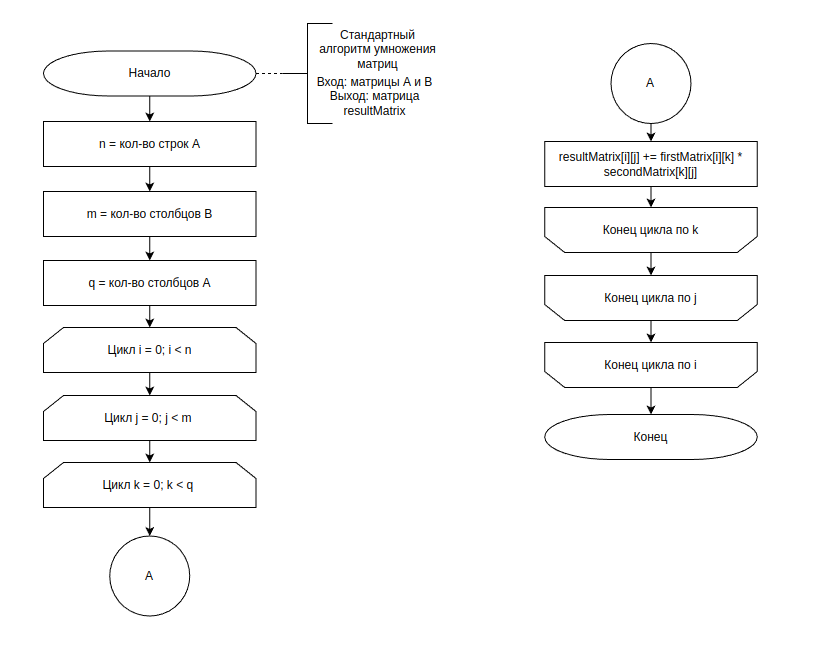
\includegraphics[scale=0.6]{photos/normal.png}}
	\caption{Схема стандартного алгоритма умножения матриц}
	
	\label{fig:normal}
\end{figure}
\FloatBarrier
\clearpage

\section{Разработка алгоритма Винограда умножения матриц}

На рисунках \ref{fig:vinograd} -- \ref{fig:vinograd2} приведена схемa рассматриваемого алгоритма.
\FloatBarrier
\begin{figure}[h]
	
	\centering{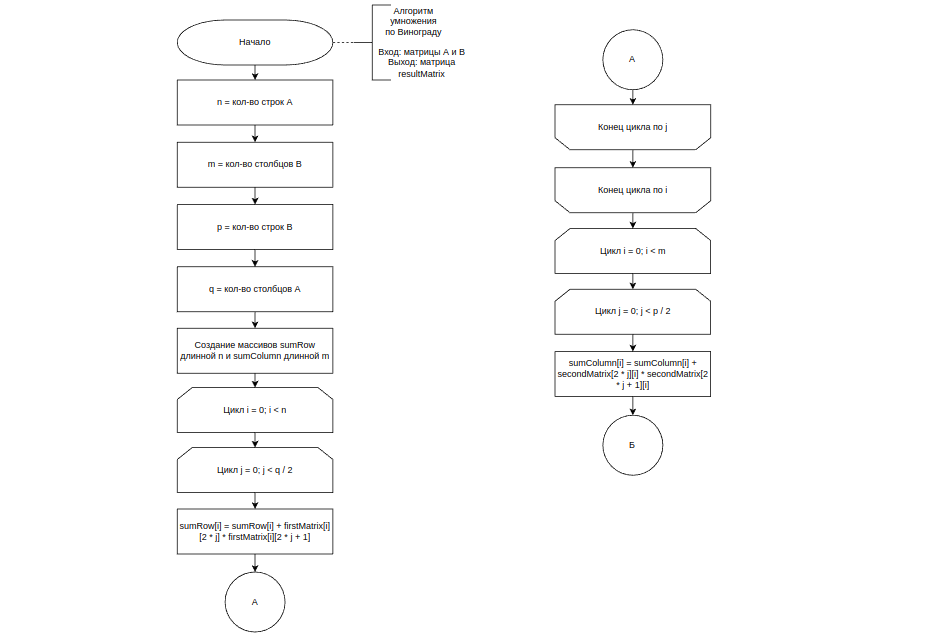
\includegraphics[scale=0.55]{photos/vinograd.png}}
	\caption{Схема алгоритма Винограда умножения матриц(Часть 1)}
	\label{fig:vinograd}
\end{figure}
\FloatBarrier

\FloatBarrier
\begin{figure}[h]
	\centering{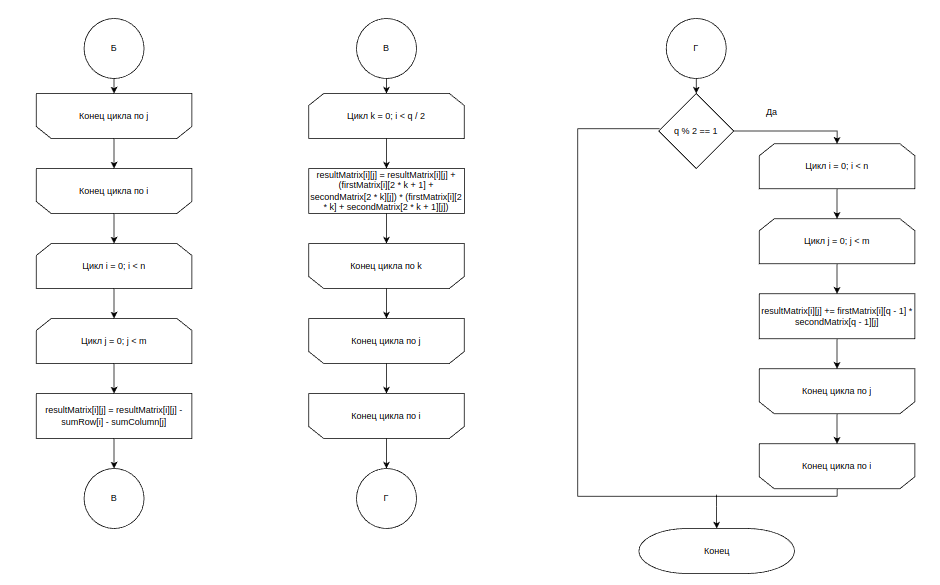
\includegraphics[scale=0.5]{photos/vinograd2.png}}
	\caption{Схема алгоритма Винограда умножения матриц(Часть 2)}
	
	\label{fig:vinograd2}
\end{figure}
\FloatBarrier
\clearpage

\section{Разработка оптимизированного алгоритма Винограда умножения матриц}

На рисунках \ref{fig:optvinograd} -- \ref{fig:optvinograd2} приведена схемa рассматриваемого алгоритма.
\FloatBarrier
\begin{figure}[h]
	\centering{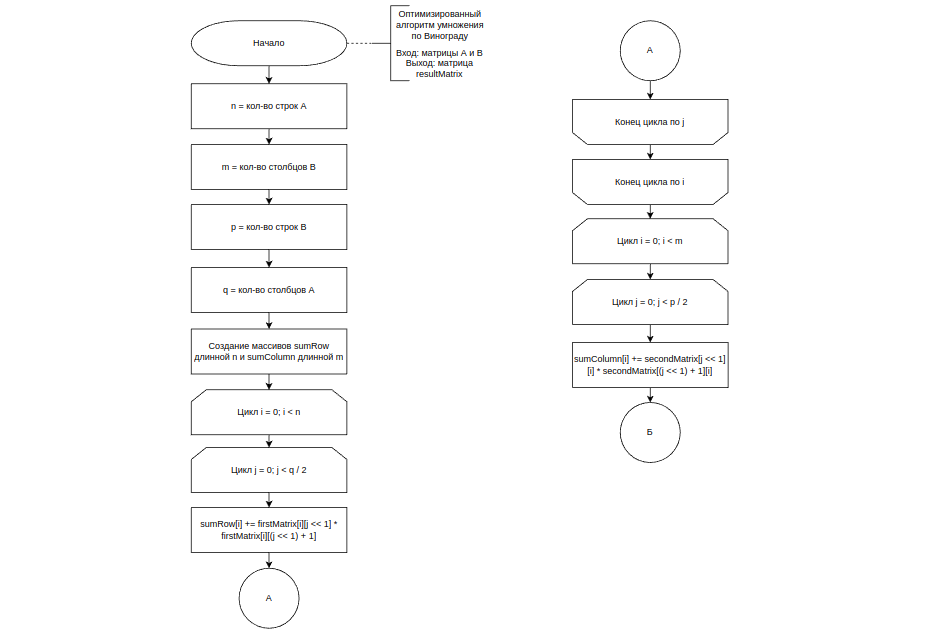
\includegraphics[scale=0.6]{photos/optvinograd1.png}}
	\caption{Схема оптимизированного алгоритма Винограда умножения матриц(Часть 1)}
	\label{fig:optvinograd}
\end{figure}
\FloatBarrier
\FloatBarrier
\begin{figure}[h]
	\centering{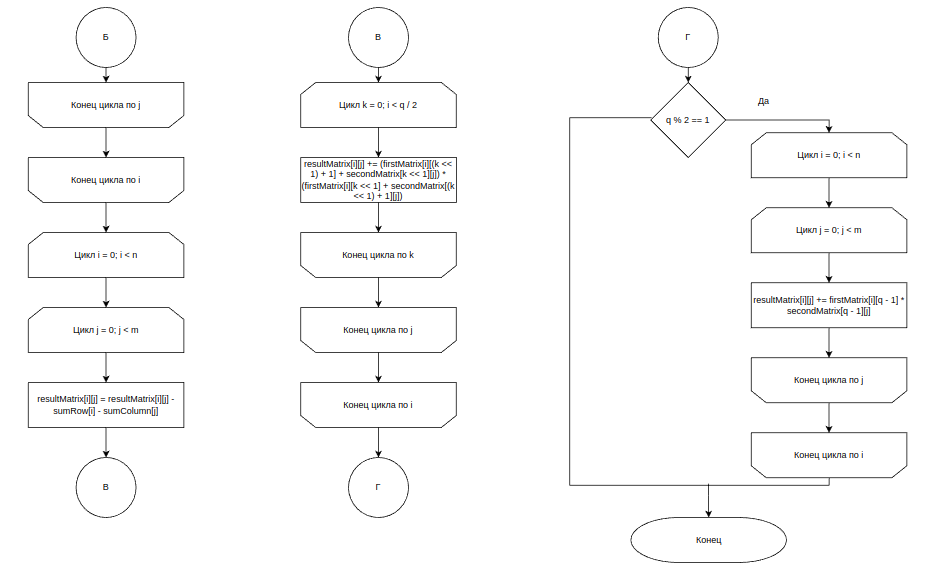
\includegraphics[scale=0.5]{photos/optvinograd2.png}}
	\caption{Схема оптимизированного алгоритма Винограда умножения матриц(Часть 2)}
	\label{fig:optvinograd2}
\end{figure}
\FloatBarrier
\clearpage
\section{Разработка алгоритма Штрассена умножения матриц}

На рисунках \ref{fig:shtrasen} -- \ref{fig:shtrasen2} приведена схема рассматриваемого алгоритма.
\FloatBarrier
\begin{figure}[h]
	
	\centering{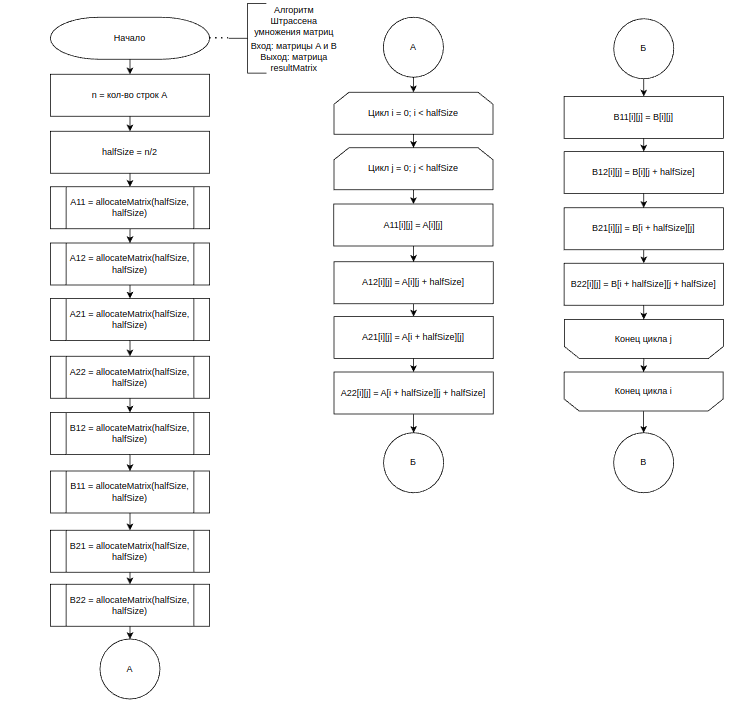
\includegraphics[scale=0.6]{photos/Shtrassen1.png}}
	\caption{Схема алгоритма Штрассена умножения матриц(Часть 1)}
	\label{fig:shtrasen}
\end{figure}
\FloatBarrier

\FloatBarrier
\begin{figure}[h]
	
	\centering{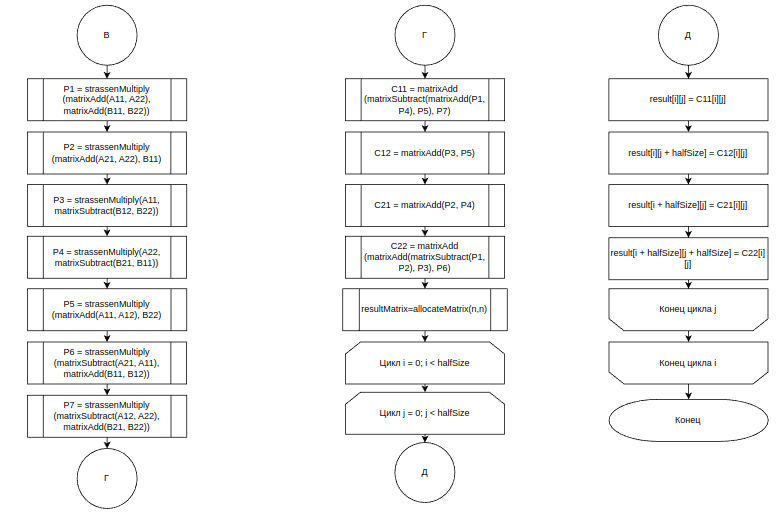
\includegraphics[scale=0.5]{photos/Shtrassen2.png}}
	\caption{Схема алгоритма Штрассена умножения матриц(Часть 2)}
	\label{fig:shtrasen2}
\end{figure}
\FloatBarrier

\section{Модель вычислений}
Для дальнейшего анализа трудоемкости необходимо ввести модель вычислений.

Операции из списка (\ref{for:opers}) имеют трудоемкость 1.

\begin{equation}
	\label{for:opers}
	=, +=, -=, +, -, ==, !=, <, >, <=, >=, [], ++, {-}-
\end{equation}

Операции из списка (\ref{for:opers2}) имеют трудоемкость 2.
\begin{equation}
	\label{for:opers2}
	*, /, \%
\end{equation}

Трудоемкость оператора выбора \code{if условие then A else B} рассчитывается как:
\begin{equation}
	\label{for:if}
	f_{if} = f_{\text{условия}} +
	\begin{cases}
		f_A, & \text{если условие выполняется,}\\
		f_B, & \text{иначе.}
	\end{cases}
\end{equation}

Трудоемкость цикла рассчитывается как:
\begin{equation}
	\label{for:for}
	f_{for} = f_{\text{инициализации}} + f_{\text{сравнения}} + N(f_{\text{тела}} + f_{\text{инкремента}} + f_{\text{сравнения}})
\end{equation}

Трудоемкость вызова функции равна 0.

\section{Трудоемкость алгоритмов}
В каждом из представленных алгоритмов создается дополнительная матрица, в которую затем записывается результат умножения. 
Необходимо отметить, что в рассмотрении трудоемкости не уделяется особого внимания этапу инициализации этой дополнительной матрицы. 
Это действие не является вычислительно сложным и не влияет значительно на общую трудоемкость алгоритмов.

\subsection{Стандартный алгоритм умножения матриц}
Трудоемкость классического алгоритма умножения матриц включает в себя следующие составляющие:

Трудоёмкость внешнего цикла по $i \in [0..M-1]$: $f = 2 + M \cdot (2 + f_{body})$.

Трудоёмкость цикла по $j \in [0..N-1]$: $f = 2 + N \cdot (2 + f_{body})$.

Трудоёмкость цикла по $k \in [0..K-1]$: $f = 2 + 11K$.

Учитывая, что сложность стандартного алгоритма равна сложности внешнего цикла, можно вычислить её, анализируя тело цикла:
\begin{equation}
	\label{for:standard}
	f_{standard} = 2 + M \cdot (4 + N \cdot (4 + 11K)) \approx 11MNK
\end{equation}

\subsection{Алгоритм Винограда умножения матриц}
Трудоёмкость алгоритма Винограда состоит из следующих составляющих.

Трудоёмкость создания и инициализации массивов MH и MV:
\begin{equation}
	\label{for:init}
	f_{init} = M + N
\end{equation}

Трудоёмкость заполнения массива MH:
\begin{equation}
	\label{for:MH}
	f_{MH} = 2 + K (2 + \frac{M}{2} \cdot 11)
\end{equation}

Трудоёмкость заполнения массива MV:
\begin{equation}
	\label{for:MV}
	f_{MV} = 2 + K (2 + \frac{N}{2} \cdot 11)
\end{equation}

Трудоёмкость цикла заполнения для чётных размеров:
\begin{equation}
	\label{for:cycle}
	f_{cycle} = 2 + M \cdot (4 + N \cdot (11 + \frac{K}{2} \cdot 23))
\end{equation}

Трудоёмкость цикла, для дополнения умножения суммой последних нечётных строки и столбца, если общий размер нечётный:
\begin{equation}
	\label{for:last}
	f_{last} = \begin{cases}
		2, & \text{размер чётный,}\\
		4 + M \cdot (4 + 14N), & \text{иначе.}
	\end{cases}
\end{equation}


Итого, для худшего случая (нечётный общий размер матриц) имеем:
\begin{equation}
	\label{for:bad}
	f =  f_{MH} + f_{MV} + f_{cycle} + f_{last}\approx 11,5 \cdot MNK
\end{equation}

Для лучшего случая (чётный общий размер матриц) имеем:
\begin{equation}
	\label{for:good}
	f =  f_{MH} + f_{MV} + f_{cycle} + f_{last} \approx 11,5 \cdot MNK
\end{equation}


\subsection{Оптимизированный алгоритм Винограда умножения матриц}

Трудоёмкость улучшенного алгоритма Винограда состоит из следующих составляющих.

Трудоёмкость создания и инициализации массивов MH и MV:
\begin{equation}
	\label{for:impr_init}
	f_{init} = M + N
\end{equation}

Трудоёмкость заполнения массива MH:
\begin{equation}
	\label{for:impr_MH}
	f_{MH} =  2 + K (2 + \frac{M}{2} \cdot 8)
\end{equation}

Трудоёмкость заполнения массива MV:
\begin{equation}
	\label{for:impr_MV}
	f_{MV} =  2 + K (2 + \frac{M}{2} \cdot 8)
\end{equation}

Трудоёмкость цикла заполнения для чётных размеров:
\begin{equation}
	\label{for:impr_cycle}
	f_{cycle} =2 + M \cdot (4 + N \cdot (11 + \frac{K}{2} \cdot 18))
\end{equation}

Трудоёмкость условия для дополнения умножения суммой последних нечётных строки и столбца, если общий размер нечётный:
\begin{equation}
	\label{for:impr_last}
	f_{last} = 
	\begin{cases}
		1, & \text{размер чётный,}\\
		4 + M \cdot (4 + 10N), & \text{иначе.}
	\end{cases}
\end{equation}

Итого, для худшего случая (нечётный общий размер матриц) имеем:
\begin{equation}
	\label{for:bad_impr}
	f = f_{MH} + f_{MV} + f_{cycle} + f_{last} \approx 9MNK
\end{equation}

Для лучшего случая (чётный общий размер матриц) имеем:
\begin{equation}
	\label{for:good_impr}
	f = f_{MH} + f_{MV} + f_{cycle} + f_{last} \approx 9MNK
\end{equation}

\subsection{Алгоритм Штрассена}
Для стандартного алгоритма умножения матриц трудоемкость будет слагаться из:
\begin{equation}
	\label{сomplexity:str_best}
	\begin{aligned}
		f_{best}(n) = 7 \cdot T(n/2) + O(n^{2})=O(n^{\log _{2}7})
	\end{aligned}
\end{equation}

\section*{Вывод}

На основе теоретических знаний, полученных в аналитическом разделе, были разработаны схемы алгоритмов. 
Благодаря им может быть вычислено произведение двух матриц разними способами.
